\section{Experimental evaluation}
\label{sec:evaluation}

\begin{inbrief}
The evaluation answers ten questions, from the safety of the bounds
(RQ0) to the robustness of the results to the assumptions of the
generator (RQ9), on synthetic applications that follow industrial
statistics, a small detection chain and a whole-vehicle application.
The main findings are collected in a box at the end of the section.
\end{inbrief}

\begin{description}[font=\sffamily\bfseries\color{brand},style=unboxed,leftmargin=0pt]
\item[RQ0] Are the network and end-to-end bounds safe, and how
pessimistic are they?
\item[RQ1] How many cores does the method use, how far is it from the
optimum, and how does it compare with general-purpose metaheuristics?
\item[RQ2] What does communication awareness buy, and at what cost?
\item[RQ3] How do network design choices (rate, topology, shaping,
replication) and the communication scheme (implicit or strict LET) change
end-to-end timing?
\item[RQ4] What do spatial constraints, heterogeneous cores and memory
contention cost?
\item[RQ5] How effective are the deadline-driven local search and the
sizing for a margin?
\item[RQ6] How many software updates does a platform absorb, for what
hardware cost?
\item[RQ7] What do the same functions need on a domain, hybrid or
distributed architecture?
\item[RQ8] What does each part of the method contribute, and how does the
method compare with the rules of practice?
\item[RQ9] Do the conclusions hold when the assumptions of the generator
change?
\end{description}
Two case studies (\cref{sec:cases}) and a scalability study
(\cref{sec:scalability}) complete the picture.

\subsection{Setup}
\label{sec:setup}

\paragraph{Applications.} Real automotive software is not public, so the
applications are generated from the published statistics of an industrial
engine-management software, the WATERS 2015 benchmark of Bosch
\cite{kramer2015waters} (\cref{app:generator}). A task-chain has 1 to 3
activation patterns, and each pattern 2 to 5 tasks, with the probabilities
of the benchmark. The periods are drawn with the benchmark's shares from
$\{1,2,5,10,20,50,100,200,1000\}$\,ms. Chain utilizations are log-uniform
between 0.1 and 8\,\% of the reference core, plus 2\,\% of heavy chains
(perception, planning) of up to 80\,\%. A quarter of the task-chains are
local to one zone; of the others, 60\,\% start with a sensor and 50\,\% end
with an actuator in a random zone. Task utilizations come from
UUniFast \cite{bini2005measuring}, redrawn while a task exceeds 30\,\% of
a core, messages range from 4 bytes to
16\,kB, and the end-to-end deadline is 300\,\% of the sum of the pattern
periods. The default application has 300 task-chains and 1299 tasks on
average (1242 to 1395), about the consolidated software of several domain
ECUs.

\paragraph{Protocol.} Each \emph{point} of an experiment fixes the
parameters and is run on 20 applications (\emph{instances}), the same
applications at every point. Means are shown with their 95\,\% confidence
interval, and differences between rules are paired by instance. Mapping
metrics are averaged over the feasible instances. A paired difference is
given as its mean $\pm$ the half-width of its 95\,\% Student
$t$-interval over the instances; a difference whose interval excludes
zero is called significant. RQ1 to RQ6 report \BFDU\ as the
reference packing rule and RQ7 to RQ9 \FFDU, the default of the tool;
both give almost the same cores at the default point (14.45 and 14.40,
\cref{fig:sweep}). All
results come from the open implementation,
single-threaded per design point, on an Intel Xeon at 2.1\,GHz. The 24
experiments run 9600 design points in about three minutes on two cores;
the exact formulation adds 250 instances, the metaheuristics 400 runs
(18 minutes), and the two simulators 23 flow sets and 45 mapped
applications. The user manual gives the commands that reproduce every
number.

\subsection{RQ0: the bounds against simulation}
\label{sec:validation}

The proofs of \cref{sec:analysis} carry the safety of the bounds. A
simulation can only refute a bound, never prove it, so the two simulators
are a check of the implementation and of the modelling assumptions: a
bound below an observed delay would reveal an error.

\paragraph{The network.} The Network Calculus bounds are compared with a discrete-event,
frame-level simulation of the same network. The simulator models
store-and-forward switches; credit-based shapers with the idle slopes of
the analysis; TAS gates with guard bands; strict priority with per-flow
token-bucket regulators at every switch for ATS; replication and
elimination of frames by sequence number for FRER; and a saturated
best-effort class. The flow sets are of two kinds: those of real mappings
(all four rules, a ring with three classes with and without FRER, a tree
with TAS, a tree with ATS, a custom topology with FRER, the domain and the
distributed platforms of \cref{tab:templates}), and random sets loaded to
40 to 70\,\% of every port they cross (all topologies and mechanisms). Each set is simulated in
24 release scenarios: synchronous and random offsets; uniform, extreme and
alternating jitters; best effort on and off. Two limits apply: the
simulator regulates ATS flows one by one where the analysis assumes
interleaved regulators, which can only lower the simulated delays; and
the \SI{20}{ms} horizon covers a single message of the flows of long
periods, whose worst case therefore rests on the scenarios rather than on
the length of the run.

\Cref{tab:netsim} reports the largest ratio of observed delay to bound
for each flow set. No simulated delay exceeded its bound, over 3377 flows. The
largest ratio, 0.87, is for ATS with three classes on a tree: with bursts
reset at every switch, the ATS bounds come closest to the simulated
delays. On the CBS mappings
the bounds are 1.5 to 2.3 times the worst observed delay. The factor is
larger with TAS and on the random loads, because random jitters rarely
align the bursts of many flows.

\begin{table}[t]
\centering\footnotesize
\caption{Network bounds against a frame-level simulation (24 scenarios
per flow set, \SI{20}{ms} horizon, two random seeds). Max ratio:
largest observed delay over its bound.}
\label{tab:netsim}
\setlength{\tabcolsep}{3pt}
\rowcolors{2}{brandlight}{white}
\begin{tabular}{@{}llrrc@{}}
\toprule
\rowcolor{white}
flow set & network & flows & max ratio & violations \\
\midrule
mapping \BFDU & star, CBS 1 & 129 & 0.600 & 0 \\
mapping \WFDU & star, CBS 1 & 193 & 0.452 & 0 \\
mapping \FFDU & star, CBS 1 & 129 & 0.600 & 0 \\
mapping \CADU & star, CBS 1 & 46 & 0.507 & 0 \\
mapping \FFDU & ring, CBS 3 & 128 & 0.613 & 0 \\
mapping \FFDU, FRER & ring, CBS 3 & 128 & 0.644 & 0 \\
mapping \FFDU & tree, TAS 1 & 129 & 0.233 & 0 \\
mapping \FFDU & tree, ATS 3 & 129 & 0.868 & 0 \\
mapping \FFDU, FRER & custom, CBS 3 & 128 & 0.686 & 0 \\
domain, \FFDU & tree, CBS 1 & 153 & 0.440 & 0 \\
distributed, \FFDU & star, ATS 1 & 180 & 0.559 & 0 \\
load 50\,\% & star, CBS 1 & 183 & 0.242 & 0 \\
load 70\,\% & star, CBS 1 & 275 & 0.212 & 0 \\
load 60\,\% & tree, CBS 1 & 228 & 0.096 & 0 \\
load 60\,\% & ring, CBS 1 & 248 & 0.083 & 0 \\
load 60\,\% & star, CBS 3 & 111 & 0.320 & 0 \\
load 50\,\% & star, TAS 3 & 116 & 0.204 & 0 \\
load 60\,\% & star, ATS 3 & 94 & 0.408 & 0 \\
load 60\,\% & ring, ATS 1 & 215 & 0.219 & 0 \\
load 40\,\%, FRER & ring, CBS 1 & 79 & 0.102 & 0 \\
load 40\,\%, FRER & ring, ATS 3 & 45 & 0.295 & 0 \\
load 40\,\%, FRER & custom, CBS 1 & 205 & 0.244 & 0 \\
load 40\,\%, FRER & custom, ATS 3 & 106 & 0.383 & 0 \\
\midrule
\rowcolor{white}
\textbf{all} & & \textbf{3377} & \textbf{0.868} & \textbf{0} \\
\bottomrule
\end{tabular}
\end{table}

\paragraph{The whole system.} A second, full-system simulator checks
the end-to-end bounds of \cref{sec:analysis}: the tasks on their cores
under preemptive fixed priorities, their LET tasks, and network delays
drawn between zero and their bound. Every core starts at a random phase
(the cores are not synchronized); a job reads its input when it starts and
writes its output when it ends; the LET task of the producer core copies
the last output written by its release (with strict LET, the output of the
last producer job whose period has ended), and that of the consumer core
reads, at the release of the consumer job, the last message arrived. Each
sample of the first task is tracked, by its timestamp, to the first job of
the last task that uses it. This gives an observed \emph{end-to-end
delay}, from the release of the sampling job to the end of that last job,
whose bound is $\Gamma^{\mathrm b}_\xi$ (\cref{eq:delay}), and an observed
maximum reaction time, bounded by $\Delta^{\mathrm b}_\xi$. Nine settings
(the zonal platform with \FFDU\ and \CADU, a ring with FRER and three
classes, a tree with TAS, shared-memory contention at \SI{20}{ns}, strict
LET on the star and on the ring, the domain and the hybrid platforms) are
mapped for five applications of 200 task-chains, and each
mapping is simulated in four scenarios: execution times at their WCET and
network delays at their bound, or both drawn uniformly (WCETs in $[0.5C,
C]$), with new phases every time.

No observed delay exceeded its bound, over 9000 task-chains
(\cref{fig:syssim}). The end-to-end bound is reached exactly by 3795
task-chains, all of them without an inter-ECU communication. With one,
the median observed delay is 81\,\% of the bound with implicit
communication and 94\,\% with strict LET, whose timing depends less on
the response times, and the largest is 99.4\,\% and 99.997\,\%; the
largest observed reaction time is 99.7\,\% of its bound.
The bounds are therefore attained, or nearly, in the worst case, and
pessimistic by about a fifth for a typical task-chain that crosses the
network. The network delays are drawn up to their bound here, so this
simulation checks the task-level part of the analysis, and the frame-level
simulation above the network bounds.

\begin{figure}[t]
\centering
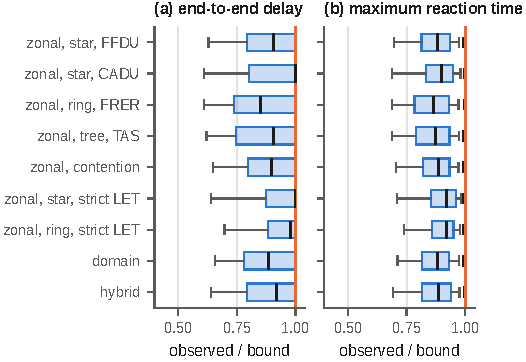
\includegraphics[width=\columnwidth]{figures/syssim}
\caption{Full-system simulation: observed delay over its bound for every
task-chain (9000 task-chains, 5 applications of 200 per setting, 4
scenarios each). Box: quartiles and median; whiskers: 5th and 95th
percentiles; tick: largest.}
\label{fig:syssim}
\end{figure}

\subsection{RQ1: number of cores and optimality gap}
\label{sec:rq1}

\paragraph{Cores and the lower bound.} \Cref{fig:sweep}(a) shows the cores
used as the sub-chain limit $\sigma$ varies, with the lower bound of
\cref{prop:lb}. \BFDU\ and \FFDU\ use 14.45 and 14.40 cores at the default point, 1.21
times the lower bound of 11.95 (1.15 to 1.36 over the instances).
Consolidation empties 1.4 cores on average. \WFDU\ spreads the load over
all 28 initial cores by construction, so its $M$ measures the spreading,
not a need. $\sigma$ barely changes the number of cores. Most task-chains
use less than 8\,\% of a core, so the cuts are mostly forced by bindings:
the fragmentation rate falls from 49\,\% at $\sigma=0.02$ to 24\,\% at
$\sigma\ge0.2$. Small sub-chains only add communications, as
\cref{fig:sweep}(b,c) shows.

\begin{figure*}[t]
\centering
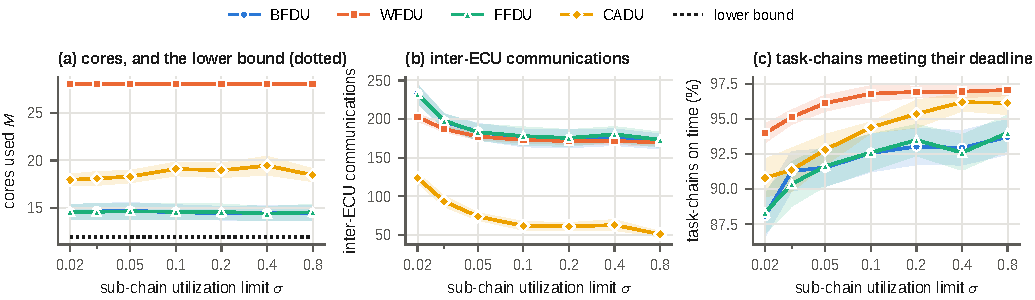
\includegraphics[width=\textwidth]{figures/sweep}
\caption{Sub-chain limit $\sigma$ and allocation rule (300 task-chains, 20
instances, 95\,\% confidence bands). \BFDU\ and \FFDU\ coincide in cores. (a) Cores
used, with the lower bound of \cref{prop:lb} (dotted). (b) Inter-ECU
communications. (c) Task-chains that meet their deadline.}
\label{fig:sweep}
\end{figure*}

\paragraph{Optimality gap.} The lower bound ignores the LET load, the
schedulability gaps and the integrality of each zone, so the ratio above
overstates the gap. The exact formulation of \cref{sec:exact} measures it.
It was run on 150 instances: 20 to 300 task-chains, 10 instances per
size, on three platforms (default; zone cores at 25\,\% speed; and 20\,\%
of replicated task-chains, 10\,\% of zone-only task-chains and 8\,MB of
memory per zone controller). On the constrained platform, no instance of
300 task-chains has an admissible mapping: the pinned tasks of some zone
alone exceed its memory, which both methods detect. Of the 140 other
instances, 134 were solved to proven optimality within 60\,s (5.3\,s on
average) and 6 stopped at the limit with their best solution, against
which the gap is then measured; the tool accepted every exact allocation.
The optimum is that of the sub-chains of step 1, without contention, over
the candidate cores of \cref{sec:exact}. \CADU\ maps only 2 of the 10
constrained instances of 200 task-chains, which \BFDU, \FFDU\ and the
exact solver all map: it fills the 8\,MB of zone memory with free
sub-chains, after which a replica finds every ECU with memory left
already running another replica of its task-chain. \Cref{fig:exact}
and \cref{tab:exact} give the result. With consolidation, \BFDU\ and
\FFDU\ are 2.3\,\% above the best allocation found on average, and equal
to it in 83\,\% of the instances. Counting only proven optima, \BFDU\ is
optimal in 113 of the 140 instances (81\,\%), and, measured against the
lower bound of the solver on the 6 unproven instances, its mean gap is at
most 2.9\,\% (2.85\,\% for \FFDU). Without consolidation they were 20\,\% above it, one to
three cores on instances that need five to twenty. The loss comes from
the order of the packing: a core opened early for a large sub-chain stays
lightly loaded, while the smaller sub-chains allocated later fill the
gaps that the pinned work leaves elsewhere; emptying such cores is what
step 3 does. \CADU\ is further from the optimum (22\,\%), on purpose: it
gives up cores to keep computations next to their devices (RQ2).

\paragraph{Other architectures.} The same study on the domain and hybrid
platforms of \cref{tab:templates} (100 more instances, all proven optimal,
in 1.4\,s on average and 11.4\,s at worst, every exact allocation
accepted by the tool; one domain instance used every candidate core of an
ECU, and solving it again with six spare cores instead of two gave the
same optimum) gives a gap of 4.4\,\% for
\BFDU\ and 4.7\,\% for \FFDU\ on the domain platform, optimal in
68\,\% and 62\,\% of the instances, and of 1.2\,\% and 1.1\,\% on the
hybrid one, optimal in 88\,\% and 90\,\% (\cref{tab:exact}). The domain
platform is the harder case: without a central computer, the free
sub-chains have no single obvious host. This study changed the method. In
its first version, a platform without a central computer gave the free
sub-chains to any ECU, in the order of the platform, which let them fill
microcontroller cores where they cost twice the utilization: on the domain
platform, \BFDU\ was 19\,\% above the optimum
on average (36 and 37\,\% at 200 and 300 task-chains) and \FFDU\
7.2\,\%. Giving them first to the ECUs with the fastest cores
(\cref{sec:other-architectures}) brought the averages down to 4.4 and
4.7\,\%. The zonal and hybrid platforms, which have a central computer,
are not affected.

\begin{figure*}[t]
\centering
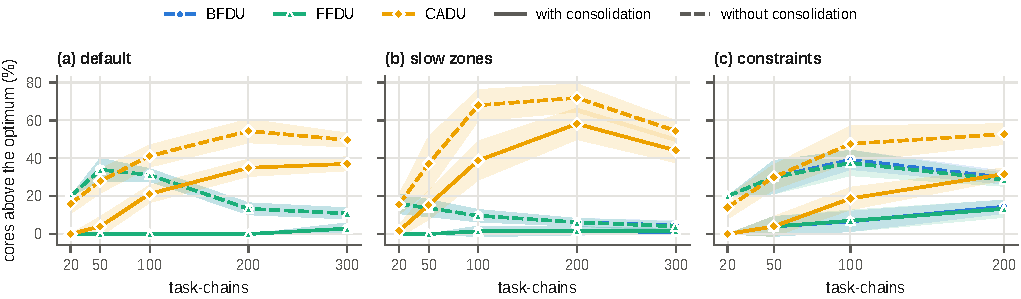
\includegraphics[width=\textwidth]{figures/exact}
\caption{Cores above the optimum found by the exact formulation (10
instances per size, 95\,\% confidence bands), with (solid) and without
(dashed) consolidation. (a) Default platform. (b) Zone cores at 25\,\%
speed. (c) Replicas, zone-only task-chains and 8\,MB of zone memory.}
\label{fig:exact}
\end{figure*}

\begin{table}[t]
\centering\footnotesize
\caption{Exact formulation against the heuristics (10 instances per row;
instances without an admissible mapping left out). Zonal platform:
default, slow zone controllers, spatial constraints; then the domain and
hybrid platforms of \cref{tab:templates}. \emph{proven}: solved to
optimality within 60\,s; \emph{opt.}: mean optimum (best found if not
proven); gaps in \% of the optimum, with consolidation / without.}
\label{tab:exact}
\setlength{\tabcolsep}{2pt}
\rowcolors{2}{brandlight}{white}
\begin{tabular}{@{}lrrrrrrr@{}}
\toprule
\rowcolor{white}
platform & chains & proven & $M_{\mathrm{LB}}$ & opt. & \BFDU & \FFDU &
\CADU \\
\midrule
default & 20 & 10/10 & 5.0 & 5.0 & 0 / 20 & 0 / 20 & 0 / 16 \\
default & 50 & 10/10 & 5.0 & 5.0 & 0 / 34 & 0 / 34 & 4 / 28 \\
default & 100 & 10/10 & 5.0 & 6.1 & 0 / 31 & 0 / 31 & 21 / 41 \\
default & 200 & 10/10 & 7.4 & 9.1 & 0 / 13 & 0 / 13 & 35 / 54 \\
default & 300 & 10/10 & 11.6 & 13.7 & 3 / 11 & 3 / 11 & 37 / 50 \\
slow zones & 20 & 10/10 & 5.0 & 5.2 & 0 / 16 & 0 / 16 & 2 / 16 \\
slow zones & 50 & 10/10 & 5.0 & 6.0 & 0 / 14 & 0 / 14 & 15 / 37 \\
slow zones & 100 & 9/10 & 5.4 & 8.2 & 1 / 10 & 1 / 10 & 39 / 68 \\
slow zones & 200 & 10/10 & 10.0 & 13.1 & 2 / 6 & 2 / 6 & 58 / 72 \\
slow zones & 300 & 7/10 & 15.7 & 19.5 & 1 / 5 & 1 / 4 & 44 / 54 \\
constraints & 20 & 10/10 & 5.0 & 5.0 & 0 / 20 & 0 / 20 & 0 / 14 \\
constraints & 50 & 10/10 & 5.0 & 5.0 & 4 / 30 & 4 / 30 & 4 / 30 \\
constraints & 100 & 8/10 & 5.0 & 5.9 & 7 / 39 & 7 / 38 & 19 / 48 \\
constraints & 200 & 10/10 & 7.6 & 9.1 & 14 / 30 & 13 / 29 & 32 / 53 \\
\midrule
domain & 20 & 10/10 & 5.0 & 5.0 & 0 / 14 & 0 / 0 & 0 / 4 \\
domain & 50 & 10/10 & 5.0 & 5.0 & 0 / 50 & 0 / 18 & 6 / 24 \\
domain & 100 & 10/10 & 5.0 & 5.1 & 10 / 83 & 2 / 37 & 38 / 63 \\
domain & 200 & 10/10 & 7.0 & 8.1 & 7 / 50 & 11 / 26 & 36 / 71 \\
domain & 300 & 10/10 & 10.8 & 12.4 & 5 / 34 & 11 / 34 & 26 / 53 \\
hybrid & 20 & 10/10 & 5.0 & 5.0 & 0 / 20 & 0 / 20 & 0 / 16 \\
hybrid & 50 & 10/10 & 5.0 & 5.0 & 0 / 34 & 0 / 34 & 2 / 24 \\
hybrid & 100 & 10/10 & 5.0 & 5.7 & 2 / 41 & 2 / 41 & 14 / 44 \\
hybrid & 200 & 10/10 & 7.2 & 8.7 & 1 / 19 & 1 / 19 & 30 / 49 \\
hybrid & 300 & 10/10 & 11.2 & 13.0 & 3 / 15 & 2 / 14 & 33 / 48 \\
\bottomrule
\end{tabular}
\end{table}


\paragraph{Against metaheuristics.} Simulated annealing (SA) and a
genetic algorithm (GA) solve the same problem: the same sub-chains, every
constraint and the schedulability test, with the number of cores as the
objective (\cref{app:baselines}). \Cref{fig:baselines} plots the gap to
the proven optimum against the time, on the ten default instances of each
size. The packing rules are optimal on all of them up to 200 task-chains
and 2.9\,\% above at 300, in 2 to 32\,ms. SA needs $10^6$ moves, 3.7 to
13.0\,s, to come as close (2.0, 0, 0 and 0.8\,\%); with $2\cdot10^5$
moves it stays 2.2 to 6.7\,\% above. The GA degrades with the size: 0,
3.3, 6.6 and 17.9\,\% after 100 generations, which take up to 61\,s.
On these instances the exact solver (0.27 to 6.3\,s on average on the
default platform) is faster than both metaheuristics and proves
optimality. Both metaheuristics minimize the cores only, so they are
given the deadline local search of the heuristic on their best mapping.
They then keep as many task-chains on time as the packing rules at 50
task-chains (97\,\%), and 2.6 to 6.4 points fewer beyond (88 to 89\,\% at
300, against 94\,\%).

\paragraph{The harder platforms.} The default platform is where the
packing rules are best, so \cref{tab:baselines-platforms} repeats the
comparison on the three platforms where they are furthest from the
optimum. With slow zones, the packing rules stay within 1.7\,\% of the
best allocation known, the GA within 0.9\,\% (in 4 to 44\,s), and SA is
no better than the rules (1.0 to 3.9\,\%). On the domain platform, the
packing rules are up to 11.1\,\% above (\FFDU; \BFDU\ up to 9.7\,\%),
and the GA closes most of that gap (0 to 4.0\,\%, in 7 to 77\,s), while
SA does not (up to 20\,\%). On the constrained
platform, no method is close at 200 task-chains: the packing rules are
13 to 14\,\% above the optimum, the GA 21\,\%, and SA finds no admissible
mapping on half of the instances. The exact solver handles all these
instances in 0.1 to 30\,s on average, proves 104 of the 110 optima, and
finds an allocation at least as good as every other method on every
instance. A metaheuristic therefore adds nothing on the default
platform; where the packing rules fall short, a GA run for tens of
seconds recovers most of the gap on two of the three platforms, and the
exact formulation all of it, in a comparable time. The packing rules
are the tool for exploring a design space, and the exact formulation, or
a GA beyond its reach, the tool for the final sizing.

\begin{table}[t]
\centering\footnotesize
\caption{The heuristic against the metaheuristics on the hard platforms
of \cref{tab:exact} (10 instances per size; on the constrained platform,
no instance of 300 task-chains is feasible). Gap: cores above the best
allocation known (the exact solver or any method), \%, mean; on time:
task-chains that meet their deadline, \%, with the deadline local search
applied to every method; SA: $10^6$ moves, GA: 100 generations, with
their CPU times; --: no admissible mapping found on some instances (SA on
5 of the 10 constrained instances of 200 task-chains).}
\label{tab:baselines-platforms}
\setlength{\tabcolsep}{2.4pt}
\begin{tabular}{@{}lrrrrrrrrr@{}}
\toprule
 & & \multicolumn{4}{c}{gap (\%)} & \multicolumn{2}{c}{on time (\%)} & \multicolumn{2}{c@{}}{time (s)} \\
\cmidrule(lr){3-6}\cmidrule(lr){7-8}\cmidrule(l){9-10}
chains & inst. & \BFDU & \FFDU & SA & GA & \FFDU & SA & SA & GA \\
\midrule
\rowcolor{white}\multicolumn{10}{@{}l}{\emph{slow zones}} \\
\quad 50 & 10 & 0.0 & 0.0 & 3.7 & 0.0 & 96.6 & 97.0 & 2.9 & 4.4 \\
\quad 100 & 10 & 1.4 & 1.4 & 3.9 & 0.0 & 94.4 & 92.9 & 5.0 & 12 \\
\quad 200 & 10 & 1.7 & 1.7 & 3.7 & 0.8 & 93.5 & 87.8 & 7.9 & 28 \\
\quad 300 & 10 & 1.0 & 1.5 & 1.0 & 0.9 & 92.4 & 86.3 & 9.0 & 44 \\
\rowcolor{white}\multicolumn{10}{@{}l}{\emph{constraints}} \\
\quad 50 & 10 & 4.0 & 4.0 & 0.0 & 0.0 & 96.6 & 96.4 & 2.9 & 4.8 \\
\quad 100 & 10 & 6.7 & 7.0 & 7.3 & 5.7 & 97.8 & 94.6 & 5.9 & 14 \\
\quad 200 & 10 & 14.4 & 13.3 & -- & 21.4 & 93.9 & -- & 3.8 & 21 \\
\rowcolor{white}\multicolumn{10}{@{}l}{\emph{domain}} \\
\quad 50 & 10 & 0.0 & 0.0 & 0.0 & 0.0 & 98.8 & 98.8 & 4.4 & 6.6 \\
\quad 100 & 10 & 9.7 & 2.0 & 20.0 & 4.0 & 96.0 & 97.7 & 8.6 & 19 \\
\quad 200 & 10 & 7.4 & 11.1 & 8.9 & 0.0 & 96.2 & 96.3 & 16 & 46 \\
\quad 300 & 10 & 4.9 & 10.6 & 8.2 & 2.6 & 94.4 & 92.3 & 20 & 77 \\
\bottomrule
\end{tabular}
\end{table}


\begin{figure*}[t]
\centering
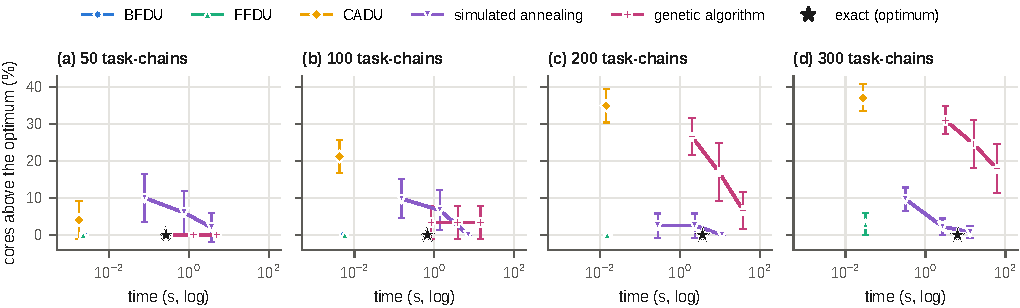
\includegraphics[width=\textwidth]{figures/baselines}
\caption{Cores above the optimum against the time to map, default
platform (10 instances per size, 95\,\% confidence intervals). The
heuristic rules with consolidation (\BFDU\ and \FFDU\ coincide),
simulated annealing with $2\cdot10^4$, $2\cdot10^5$ and $10^6$ moves,
the genetic algorithm with 5, 25 and 100 generations (CPU time), and the
exact formulation (wall time, two threads).}
\label{fig:baselines}
\end{figure*}

\begin{table}[t]
\centering\footnotesize
\caption{Time to map one application. Exact: wall time of the constraint
program (two threads, 60\,s limit), mean and worst over the three
zonal platforms of \cref{tab:exact}, and the instances proven optimal. The
others: mean CPU time on the default platform (10 instances), the
heuristic with consolidation, the simulated annealing with $10^6$ moves and
the genetic algorithm with 100 generations.}
\label{tab:speed}
\setlength{\tabcolsep}{3pt}
\rowcolors{2}{brandlight}{white}
\begin{tabular}{@{}rrrrrrrr@{}}
\toprule
\rowcolor{white}
 & \multicolumn{3}{c}{exact (s)} & \multicolumn{2}{c}{heuristic (ms)} &
 \multicolumn{2}{c@{}}{baselines (s)} \\
\cmidrule(lr){2-4}\cmidrule(lr){5-6}\cmidrule(l){7-8}
\rowcolor{white}
chains & mean & worst & proven & \FFDU & \CADU & SA & GA \\
\midrule
50 & 0.37 & 1.8 & 30/30 & 2 & 2 & 3.7 & 5.0 \\
100 & 7.83 & 60.2 & 27/30 & 6 & 4 & 7.1 & 14.2 \\
200 & 4.45 & 13.1 & 30/30 & 15 & 14 & 11.2 & 37.9 \\
300 & 17.93 & 60.9 & 17/20 & 32 & 27 & 13.0 & 61.4 \\
\bottomrule
\end{tabular}
\end{table}


\Cref{fig:architecture-results} varies the speed of the zone cores. At a
quarter of the speed of the central computer, the pinned work of the zones
needs 12.8 zone cores (\BFDU), and the task-chains lose a point of deadline
satisfaction because every response time in a zone grows. From 75\,\%
speed upwards the zones need 6 cores or fewer, and the central computer is
the bottleneck. A cheap microcontroller-class zone controller thus costs
cores in proportion to its pinned work, not to the whole application.

\begin{figure}[t]
\centering
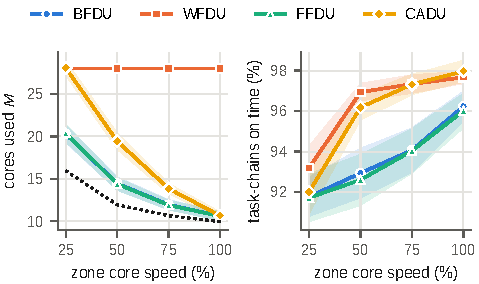
\includegraphics[width=\columnwidth]{figures/architecture}
\caption{Speed of the zone cores (central computer at 100\,\%). Left:
cores used and lower bound (dotted). Right: task-chains that meet their
deadline.}
\label{fig:architecture-results}
\end{figure}

\subsection{RQ2: communication awareness}
\label{sec:rq2}

\CADU\ keeps a computation next to the device it serves whenever the zone
has room. At the default point it removes 64\,\% of the inter-ECU
communications (63 instead of 177; paired difference $-114\pm15$). The
largest network bound falls from \SI{1.40}{ms} to \SI{0.58}{ms}, and the
share of task-chains that meet their deadline rises from 92.9 to 96.2\,\%
(paired difference $+3.3\pm1.2$ points). The price is $+5.0\pm0.4$ cores:
the work kept in the zones runs on cores at half speed, so the application
load grows from 10.2 to 13.7 cores. \Cref{fig:tradeoff} shows the
trade-off for every instance. \BFDU\ and \FFDU\ are the cheapest. \CADU\
dominates \WFDU\ in cores, at almost the same deadline satisfaction.
\WFDU's good timing comes from spreading: every core is lightly loaded and
response times are short. Affinity (trying the cores of the same
task-chain first) removes all communications between cores of one ECU for
\WFDU, but changes the bin-packing rules by less than 0.5 point, because
those rules already pack the sub-chains of a task-chain together.

\begin{figure}[t]
\centering
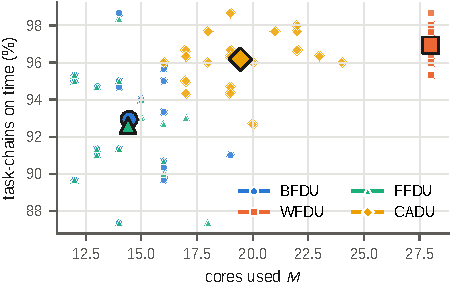
\includegraphics[width=\columnwidth]{figures/tradeoff}
\caption{Cores against task-chains that meet their deadline, every
instance of the default point (small markers) and means (large markers):
\CADU\ trades cores for deadline satisfaction.}
\label{fig:tradeoff}
\end{figure}

\subsection{RQ3: network design and communication}
\label{sec:rq3}

\paragraph{Rate, preemption, message sizes.} \Cref{fig:network}(a,b)
varies the link rate, frame preemption and the message sizes. At
100\,Mbit/s, the port of the central computer carries all the traffic
between zones in a bin-packed mapping: its load reaches 57\,\%, and only
75\,\% of the task-chains meet their deadline, against 95\,\% with \CADU,
whose port load is three times lower. With a third of the messages large
(up to 64\,kB, a sensor-heavy application), even 1\,Gbit/s overloads that
port with bin packing (69\,\% load, close to the 75\,\% idle slope, and
some ports above it): 73\,\% of the task-chains meet their deadline,
against 95\,\% with \CADU. Frame preemption changes almost nothing,
because the blocking of one best-effort frame (\SI{12}{\micro s} at
1\,Gbit/s) is small next to the LET sampling delays of milliseconds.

\begin{figure*}[t]
\centering
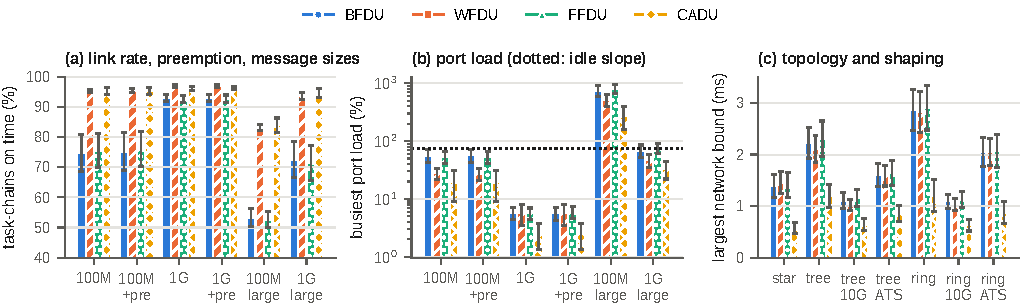
\includegraphics[width=\textwidth]{figures/network}
\caption{Network design. (a) Task-chains that meet their deadline and (b)
busiest port load (log scale; above the idle slope, flows have no bound),
for link rates of 100\,Mbit/s and 1\,Gbit/s, with frame preemption (+pre)
and with large sensor messages. (c) Largest network bound for the three
topologies, with a 1 or 10\,Gbit/s backbone, and with ATS instead of CBS.}
\label{fig:network}
\end{figure*}

\paragraph{Topology and shaping.} \Cref{fig:network}(c) compares
topologies at the default load. A tree or a ring adds switch ports to the
routes, which raises the largest bound from \SI{1.4}{ms} (star) to
\SI{2.2}{ms} (tree) and \SI{2.9}{ms} (ring) with \BFDU. On the ring, the
cyclic dependencies make the bursts grow around the ring. ATS cuts this
growth: the regulators reset the bursts at every switch, and the largest
bound falls to \SI{1.6}{ms} on the tree and \SI{2.0}{ms} on the ring, with
the same 1\,Gbit/s links. A 10\,Gbit/s backbone brings both topologies
near \SI{1.1}{ms}. Deadline satisfaction moves by less than one point: at
this load, LET sampling, not the network, dominates the reaction times.

\paragraph{Frame replication.} \Cref{fig:frer-results} adds FRER on the ring for
10 to 30\,\% of replicated task-chains. Replication sends a second member
stream around the other side of the ring, so the busiest backbone link
carries up to 1.4 points more load, and the largest bound grows by about
2\,ms with CBS (from 2.1 to 4.1\,ms at 30\,\%) and by 1.4\,ms with ATS (from
1.5 to 2.9\,ms). The bound of a replicated flow is that of its longer
route, and the burst after the elimination grows with the difference
between the two routes (\cref{prop:frer}). Deadline satisfaction drops by
at most 0.4 point. Making the redundancy of the replicated task-chains
survive a link or switch failure therefore costs little at this load, and
less with ATS than with CBS, since the member streams do not accumulate
bursts around the ring.

\begin{figure}[t]
\centering
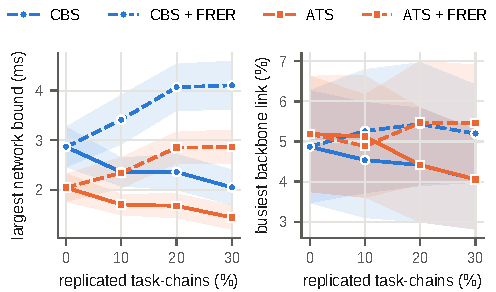
\includegraphics[width=\columnwidth]{figures/frer}
\caption{Frame replication on the ring (\BFDU): largest network bound and
busiest backbone link, with CBS or ATS, against the share of replicated
task-chains.}
\label{fig:frer-results}
\end{figure}

\paragraph{Implicit communication or strict LET.} \Cref{tab:communication}
maps the same applications with the two schemes of
\cref{sec:execution}. The cores do not change, and the allocation barely
does: only the local search, which sees other deadlines, moves a few
sub-chains. Strict LET removes the response time from the release
jitter of every flow ($J_h=C^{\LET}$ instead of $R_{\mathrm{prod}}+
T^{\LET}$), so the largest network bound falls by 19\,\% with \FFDU\ (by
270\,\si{\micro s} $\pm$ 80) and by 15\,\% on the ring. But every
crossing between cores now waits for the end of the period of its
producer, so the mean reaction bound grows by 39\,ms with \FFDU\ (by 19\,\%)
and by 16\,ms with \CADU, and the task-chains on time drop by 30 points
with \FFDU\ and 16 with \CADU\ ($\pm$ 2.2 and 1.4). The cause is
structural: a single-pattern task-chain of period $T$ with $c$ crossings
has a reaction bound of at least $(c+1)T$ with implicit communication
and $(2c+1)T$ with strict LET, so a deadline of $3T$ admits one crossing
with the first and none with the second. With deadlines at 500\,\% the gap
narrows to 4.2 and 1.5 points. The determinism of strict LET is therefore
paid in deadlines, and the fewer crossings of \CADU\ halve the bill:
strict LET needs a communication-aware allocation, or deadlines set for
it.

\begin{table}[t]
\centering\footnotesize
\caption{Implicit communication or strict LET between cores (300
task-chains, 20 instances). on time: task-chains that meet their deadline
(\%); $\bar\Delta$: mean bound of the maximum reaction time (ms); $d$:
largest network bound (\si{\micro s}).}
\label{tab:communication}
\setlength{\tabcolsep}{2.6pt}
\begin{tabular}{@{}lrrrrrr@{}}
\toprule
 & \multicolumn{3}{c}{\FFDU} & \multicolumn{3}{c@{}}{\CADU} \\
\cmidrule(lr){2-4}\cmidrule(l){5-7}
 & on time & $\bar\Delta$ & $d$ & on time & $\bar\Delta$ & $d$ \\
\midrule
\rowcolor{white}\multicolumn{7}{@{}l}{\emph{default point}} \\
\quad implicit & 92.6 & 205.6 & 1415 & 96.2 & 191.2 & 578 \\
\quad strict LET & 62.4 & 244.6 & 1145 & 79.7 & 207.0 & 402 \\
\rowcolor{white}\multicolumn{7}{@{}l}{\emph{deadlines at 500\,\%}} \\
\quad implicit & 99.5 & 208.9 & 1496 & 99.6 & 195.6 & 573 \\
\quad strict LET & 95.3 & 246.6 & 1109 & 98.1 & 222.4 & 435 \\
\rowcolor{white}\multicolumn{7}{@{}l}{\emph{ring, three classes}} \\
\quad implicit & 91.3 & 208.7 & 37135 & 96.0 & 191.7 & 40615 \\
\quad strict LET & 61.7 & 248.5 & 31650 & 79.3 & 207.5 & 35916 \\
\bottomrule
\end{tabular}
\end{table}


\paragraph{The whole vehicle.} On the whole vehicle (\cref{tab:vehicle},
2000 task-chains), the network matters more. Raising the backbone and the
link of the central computer to 10\,Gbit/s increases the task-chains that
meet their deadline from 81.4 to 88.3\,\% (\BFDU). Splitting the LET
traffic into classes by period does not help with CBS. With two classes,
the low class (periods above 20\,ms) gets bounds of up to \SI{99}{ms}, and
deadline satisfaction falls to 83\,\%. Three classes with proportional idle
slopes (\cref{eq:slopes}) recover 88.8\,\%, close to one class. TAS with
one window is close to CBS (88.0\,\%); with three windows it loses four
points, because each class only gets its own window. ATS gives the lowest
bounds with one class (\SI{2.8}{ms}, against \SI{3.9}{ms} for CBS) and
also with three (\SI{3.1}{ms}, against \SI{36}{ms}), and the best deadline
satisfaction (89.0\,\% with three classes).

\subsection{RQ4: spatial constraints, core types and contention}
\label{sec:rq4}

\paragraph{Spatial constraints.} \Cref{fig:constraints}(a) adds constraints
one at a time. Replicating 10 to 30\,\% of the task-chains with ECU
separation costs at most 0.5 core (\BFDU). The replicas replace other
task-chains, so that the application keeps its number of task-chains, and
only task-chains that are not heavy are replicated; the applications with
replicas are therefore slightly lighter than those without, and this
figure compares the two only roughly. Two replicas may not share the
central computer, so one of each pair runs in a zone (central cores fall
from 6.7 to 4.7, zone cores rise from 7.8 to 10.2), mostly on zone cores
that were already there. Separating replicas by core only needs 13.7 cores instead
of 14.6, but it puts both replicas on the central computer, where one
failure of that ECU loses both. Forbidding
the central computer to 20\,\% of the task-chains (zone-only safety
functions) costs 1.2 cores. Co-location of 30\,\% of consecutive free tasks
costs nothing measurable. A memory of 8\,MB per zone controller makes 55\,\%
of the applications infeasible. In all of them, the pinned tasks of some
zone alone exceed 8\,MB, which no mapping can fix; by
\cref{prop:memory}, and because a free sub-chain can always go to a new
core of the central computer here, this is the only possible cause.

\begin{figure*}[t]
\centering
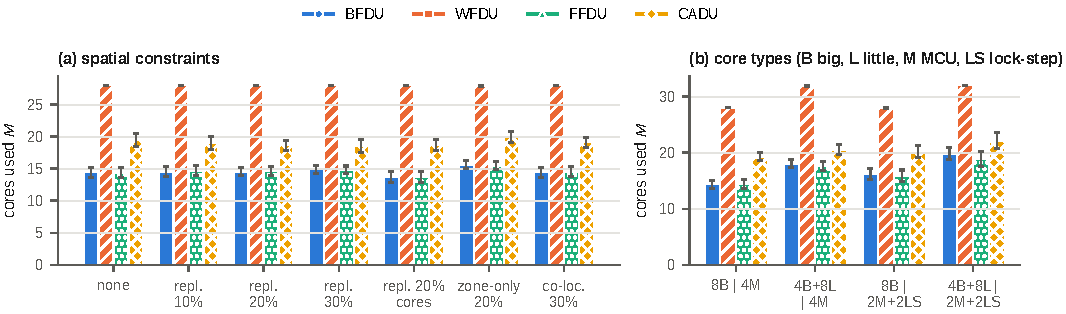
\includegraphics[width=\textwidth]{figures/constraints}
\caption{Cores used under (a) spatial constraints and (b) heterogeneous
core types, with every WCET within $\pm30\,\%$ of its speed ratio on each
type (B: big, L: little, M: MCU, LS: lock-step; 10\,\% of the task-chains
on lock-step cores when LS cores exist).}
\label{fig:constraints}
\end{figure*}

\paragraph{Core types.} \Cref{fig:constraints}(b) varies the core types,
with per-type WCET factors drawn within $\pm30\,\%$ of the speed ratio.
Replacing half of the big cores of the central computer by twice as many
little ones (40\,\% speed) adds 3.7 cores for \BFDU. Replacing half of
the zone cores by lock-step cores, for the 10\,\% of safety task-chains
that need them, adds 1.8 cores; both
together add 5.5 cores (19.8 instead of 14.4). Splitting the zone cores
between safety and other work removes packing flexibility in every zone.
This cost of dedicated safety hardware is visible only with a type-aware
model.

\paragraph{Memory contention.} \Cref{fig:contention} sets the latency of a
memory request from 0 to 100\,ns, with 1000 requests per millisecond of
WCET. At 100\,ns a request may wait \SI{0.3}{\micro s} on a zone
controller of four cores and \SI{0.7}{\micro s} on the central computer of
eight (more when cores are added there), a contention of 30 to 70\,\% of the reference WCET. The application
load grows from 10.2 to 15.0 cores, and \BFDU\ needs 22.2 cores instead of
14.4 (+54\,\%). \CADU\ suffers less (+22\,\%, from 19.5 to 23.7 cores),
because its zone cores run at half speed, so the same wait is a smaller
share of their WCETs, and its central computer uses few cores. The gap
between packing and communication awareness thus shrinks from five cores
to 1.5. Ignoring contention, as WCET-inclusive models do, would hide that
the number of cores a heavily loaded central computer needs grows with
the cores themselves.

\begin{figure}[t]
\centering
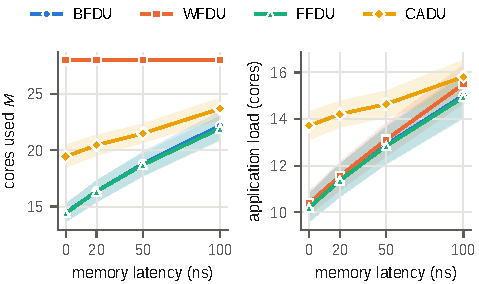
\includegraphics[width=\columnwidth]{figures/contention}
\caption{Shared-memory contention: cores used and application load
against the latency of a memory request (1000 requests per ms of WCET,
round robin).}
\label{fig:contention}
\end{figure}

\subsection{RQ5: deadline local search and margins}
\label{sec:rq5}

\paragraph{Local search.} \Cref{fig:deadlines} varies the deadline from 200
to 600\,\% of the sum of the pattern periods. At the default 300\,\%,
without the local search, the bin-packing rules leave 88.8\,\% of the
task-chains on time; the local search raises this to 92.9\,\% with 12 kept
moves, in \SI{6}{ms} of CPU time per design point. It is most effective
where cores have room: it lifts \WFDU\ from 79 to 97\,\% at 300\,\% and
from 49 to 87\,\% at 200\,\%, while \BFDU\ only goes from 55 to 60\,\% at
200\,\%: tightly packed cores leave little room for the moves. No move can
remove a communication between two pinned sub-chains in different zones, so
a task-chain whose deadline is shorter than the sampling delays of such
communications stays late (\cref{sec:example}).

\begin{figure}[t]
\centering
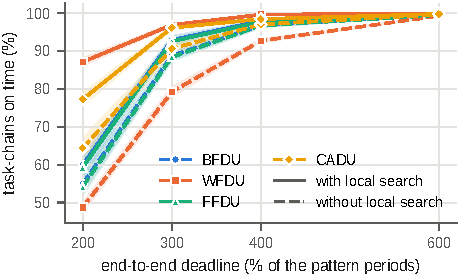
\includegraphics[width=\columnwidth]{figures/deadlines}
\caption{End-to-end deadline, with (solid) and without (dashed) the
deadline-driven local search.}
\label{fig:deadlines}
\end{figure}

\paragraph{LET cost and utilization cap.} The LET cost scales with
$c_{\LET}$. At \SI{200}{\micro s} the LET tasks load 4.6 cores, and \BFDU\
needs 18.9 cores instead of 14.4. The utilization cap sets the margin:
from $\varphi=1$ to $0.6$, the critical scaling factor grows from 1.00 to
1.67, while the cores grow from 11.5 to 21.2 (\BFDU). At $\varphi=1$,
0.7\,\% of the cores are unschedulable after priority assignment, and the
relocation moves repair all of them.

\paragraph{Margins.} \Cref{fig:margins} compares two ways to obtain a
margin on the real WCETs. A WCET margin of $m$\,\% inflates every WCET and
gives the factor $\lambda(1+m/100)$ on the real WCETs. Sizing for
$\lambda^\star$ (\cref{sec:sizing}) lowers $\varphi$ instead. For the same
guaranteed factor, both need about the same number of cores: 18.3 cores for
a 20\,\% margin (factor 1.49) and 18.5 for $\lambda^\star=1.5$ (\BFDU).
Sizing, however, guarantees the target directly and reports it, runs at
most nine design points, and keeps the real WCETs for every other metric.

\begin{figure}[t]
\centering
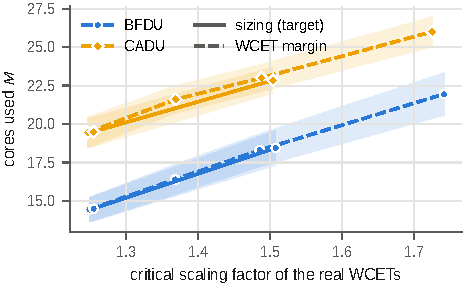
\includegraphics[width=\columnwidth]{figures/margins}
\caption{Cores against the critical scaling factor guaranteed on the real
WCETs: WCET margins of 0, 10, 20, 40\,\% (dashed) and sizing for targets
1.1, 1.25, 1.5 (solid).}
\label{fig:margins}
\end{figure}

\subsection{RQ6: the life of a platform}
\label{sec:rq6}

\Cref{fig:lifecycle} sizes the platform at the SOP for 300 task-chains with
a provisioning cap $\varphi_{\mathrm{SOP}}$ from 0.5 to 0.8, then adds ten
software updates of 15 task-chains each (+50\,\% of software in all) up to
the design cap of 0.8. A platform sized at the design cap absorbs no update
with \BFDU: its cores are full, and the new pinned drivers need room in
their zones. Every step of provisioning buys updates: 1.3 updates at
$\varphi_{\mathrm{SOP}}=0.7$ for 2.8 more cores, 3.8 at 0.6 for 6.8 more,
and 6.5 at 0.5 for 12.1 more (26.6 cores). The relation is close to linear
in the cores, about one update for two cores here. \WFDU\ is a special
case: in these experiments it uses all 28 initial cores (29 at
$\varphi_{\mathrm{SOP}}=0.5$), and so absorbs
about five updates whatever the cap, but at a cost close to that of the
most provisioned \BFDU\ platform. \CADU\ absorbs updates at the price of
its extra cores, with the best deadline satisfaction along the life (96\,\%
against 91--93\,\%). The critical scaling factor of a \BFDU\ platform
falls to 1.26--1.39 after the first update and to about 1.26 after the
second, whatever its provisioning (\cref{fig:lifecycle}(b)):
an update fills some core up to the design cap, and the factor of the
platform is that of its fullest core. Provisioning therefore buys
updates, not margin.

\begin{figure}[t]
\centering
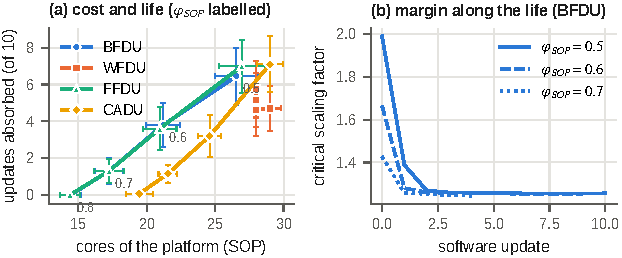
\includegraphics[width=\columnwidth]{figures/lifecycle}
\caption{Life of a platform: (a) cores bought at the SOP against the
software updates absorbed (of ten updates of 15 task-chains), for
$\varphi_{\mathrm{SOP}}$ from 0.5 to 0.8; (b) critical scaling factor
after each update (\BFDU), averaged over the platforms that have absorbed
every update so far.}
\label{fig:lifecycle}
\end{figure}

\subsection{RQ7: other E/E architectures}
\label{sec:rq7}

\Cref{fig:dse} maps the same applications (the same generator seeds) of
100 to 300 task-chains onto the four platforms of \cref{tab:templates}.
The sensors and actuators are wired to the ECUs that are not central
computers, so the bindings follow each architecture: five zone
controllers in the zonal platform, five domain controllers in the domain
one, the ADAS controller and the four zones in the hybrid one, all twelve
ECUs in the distributed one.

\paragraph{Cores.} At 300 task-chains the hybrid platform needs the
fewest cores with \FFDU\ (13.2, lower bound 11.4), then the domain one
(13.35, 11.1) and the zonal one (14.4, 11.95); the ratio to the lower
bound is 1.16, 1.20 and 1.21. Both alternatives save about a core over
the zonal platform for the same reason: part of the pinned work runs on
ECUs with big cores, a fifth of it on the ADAS controller of the hybrid
platform and two fifths on the ADAS and infotainment controllers of the
domain one, instead of on microcontroller cores at half speed, which
lowers the bound itself. The distributed platform runs out of room. It needs at least one
core per ECU (12), and with at most two cores per small ECU and four on
the ADAS controller, \FFDU\ maps 95\,\% of the applications of 200
task-chains and 50\,\% of those of 300 (\CADU: 100 and 75\,\%). The
failures are sub-chains that find every allowed ECU at its largest number
of cores; placing the bound sub-chains before the free ones, so that
these cannot take the cores of the ADAS controller, maps fewer
applications, not more. Its 100\,Mbit/s network is the most loaded
(23\,\% on the busiest port at 300 task-chains with \FFDU, against at
most 6\,\% elsewhere).

\paragraph{Communications and timing.} At 300 task-chains, \FFDU\ creates
166 to 180 inter-ECU communications on the three platforms that map every
application, and \CADU\ 62 to 74: a reduction of 65\,\% on the zonal
and hybrid platforms and of 56\,\% on the domain one. The
share of task-chains on time is within one point between them (92.6 to
93.1\,\% with \FFDU, 96.2 to 96.7\,\% with \CADU). The zonal platform is
therefore not the cheapest in cores for this software: what matters most
is the speed of the cores that run the pinned work.

\begin{figure*}[t]
\centering
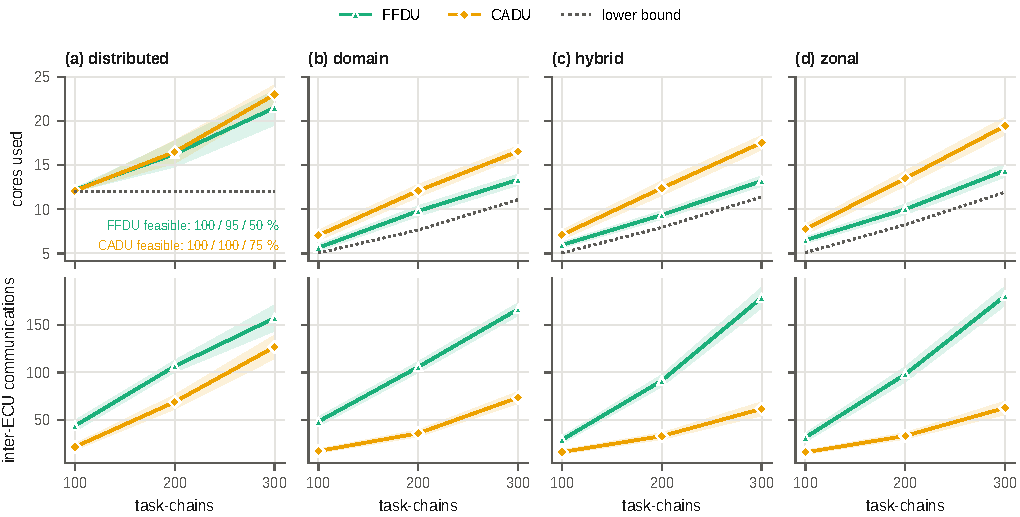
\includegraphics[width=\textwidth]{figures/dse}
\caption{The same applications on four E/E architectures
(\cref{tab:templates}; 20 instances, 95\,\% confidence bands, means over
the feasible instances). Top: cores used and lower bound (dotted).
Bottom: inter-ECU communications. Only the distributed platform has
instances without an admissible mapping; their share is given in (a), and
its means are over fewer, different instances for each rule and size.}
\label{fig:dse}
\end{figure*}

\subsection{RQ8: ablation and the rules of practice}
\label{sec:rq8}

\paragraph{Ablation.} \Cref{tab:ablation} removes one part of the method
at a time, on the default point and on a stressed one ($\varphi=1$, so
that some cores are unschedulable after step 4, and deadlines at
200\,\%). Consolidation saves $1.40\pm0.28$ cores with \FFDU\ and
$1.85\pm0.35$ with \CADU\ (default), and $0.90\pm0.21$ and $1.50\pm0.32$
(stressed). The cores it empties also leave less room, so without it
$3.65\pm1.19$ points more task-chains are on time with \FFDU\ (default).
The deadline-driven local search adds $4.18\pm0.96$ points of task-chains
on time with \FFDU\ and $5.50\pm1.37$ with \CADU\ (default), and
$4.60\pm1.26$ and $12.83\pm2.44$ (stressed), without changing the cores.
The relocation moves only matter when cores are unschedulable: in the
stressed setting, 0.7\,\% of the cores of \FFDU\ are unschedulable after
the priority assignment, and without relocation they stay so (the
apparent saving of $0.20\pm0.19$ cores is that of a mapping that is not
admissible). Adding the swap moves of the first version of step 5 before
the relocation moves changed no result in either setting, nor in any other
experiment (\cref{sec:placement}); they are now an option, off by
default. Affinity makes no significant difference to the packing rules
(every paired interval contains zero). Without all of them, \FFDU\ needs $1.40\pm0.28$
more cores and loses $6.58\pm1.11$ points of task-chains on time
(default), and $15.45\pm2.28$ points when stressed.

\begin{table*}[t]
\centering\footnotesize
\caption{Ablation: the method with one part removed (300 task-chains, 20
instances). Default: the default platform. Stressed: utilization cap
$\varphi=1$ and deadlines at 200\,\% of the sum of the pattern periods.
$M$: cores used; on time: task-chains that meet their deadline (\%);
sched.: cores schedulable at the end (\%, \FFDU).}
\label{tab:ablation}
\setlength{\tabcolsep}{4pt}
\rowcolors{2}{brandlight}{white}
\begin{tabular}{@{}lrrrrrrrrrr@{}}
\toprule
\rowcolor{white}
 & \multicolumn{5}{c}{default} & \multicolumn{5}{c@{}}{stressed} \\
\cmidrule(lr){2-6}\cmidrule(l){7-11}
\rowcolor{white}
 & \multicolumn{2}{c}{\FFDU} & \multicolumn{2}{c}{\CADU} & &
 \multicolumn{2}{c}{\FFDU} & \multicolumn{2}{c}{\CADU} & \\
\rowcolor{white}
variant & $M$ & on time & $M$ & on time & sched. & $M$ & on time & $M$ &
on time & sched. \\
\midrule
full method & 14.40 & 92.6 & 19.45 & 96.2 & 100.0 & 11.45 & 61.3 & 16.15 & 80.9 & 100.0 \\
no affinity & 14.40 & 92.6 & 19.40 & 96.2 & 100.0 & 11.45 & 61.2 & 16.20 & 80.7 & 100.0 \\
no consolidation & 15.80 & 96.2 & 21.30 & 97.9 & 100.0 & 12.35 & 57.1 & 17.65 & 87.0 & 100.0 \\
with swap moves & 14.40 & 92.6 & 19.45 & 96.2 & 100.0 & 11.45 & 61.3 & 16.15 & 80.9 & 100.0 \\
no relocation moves & 14.40 & 92.6 & 19.45 & 96.2 & 100.0 & 11.25 & 60.7 & 15.95 & 80.8 & 99.3 \\
no local search & 14.40 & 88.4 & 19.45 & 90.7 & 100.0 & 11.45 & 56.7 & 16.15 & 68.1 & 100.0 \\
none of them & 15.80 & 86.0 & 21.30 & 90.7 & 100.0 & 12.30 & 45.6 & 17.55 & 68.6 & 99.3 \\
\bottomrule
\end{tabular}
\end{table*}


\paragraph{Rules of practice.} \Cref{tab:practice} compares the method
with three rules a practitioner might apply. Keeping task-chains whole,
cut only where their bindings force it ($\sigma=\varphi$), costs no
significant core ($+0.15\pm0.23$), and keeps $1.40\pm1.06$ points more
task-chains on time with $7.2\pm6.1$ fewer communications on this point;
the next paragraph shows where it fails. Putting all free software on the
central computer costs $0.75\pm0.40$ cores, adds $55\pm10$ inter-ECU
communications (+31\,\%) and loses $6.93\pm1.01$ points of task-chains on
time: the zone cores that the pinned work leaves partly empty are not used
for nearby computations. On this point, applying both rules gives the
cores and communications of the central rule alone. Balancing the load (\WFDU) spreads the software
over all 28 initial cores ($+13.6\pm0.8$) for $4.33\pm1.38$ points more on
time. \CADU\ gets most of this timing benefit ($+3.58\pm1.35$ points) for
$5.05\pm0.49$ more cores, and removes two thirds of the communications.

\begin{table}[t]
\centering\footnotesize
\caption{The method against the rules of practice (300 task-chains, 20
instances). $M$: cores used, on the central computer / the zone
controllers; hops: inter-ECU communications; port: load of the busiest
port (\%); on time: task-chains that meet their deadline (\%).}
\label{tab:practice}
\setlength{\tabcolsep}{2.6pt}
\rowcolors{2}{brandlight}{white}
\begin{tabular}{@{}lrrrrr@{}}
\toprule
\rowcolor{white}
rule & $M$ & central/zones & hops & port & on time \\
\midrule
method, \FFDU & 14.40 & 6.65/7.75 & 180.3 & 5.6 & 92.6 \\
method, \CADU & 19.45 & 1.85/17.60 & 62.9 & 2.6 & 96.2 \\
whole task-chains & 14.55 & 6.70/7.85 & 173.2 & 5.2 & 94.0 \\
central computer only & 15.15 & 8.30/6.85 & 235.6 & 9.2 & 85.7 \\
whole and central only & 15.15 & 8.30/6.85 & 235.6 & 9.2 & 86.0 \\
load balancing (\WFDU) & 28.00 & 8.00/20.00 & 171.6 & 5.7 & 96.9 \\
\bottomrule
\end{tabular}
\end{table}


\paragraph{The sub-chain limit.} \Cref{tab:limit} raises $\sigma$ from
0.4 to 0.6 and to $\varphi=0.8$ (whole task-chains). On the default point,
most task-chains are far smaller than $\sigma$ (RQ1), so the limit cuts
little more than the bindings do: a larger $\sigma$ changes the cores of
\FFDU\ by no significant amount, and saves \CADU\ $1.00\pm0.64$ cores
and $12.0\pm5.1$ communications at $\sigma=0.8$. The limit matters when a
sub-chain grows after the cut. With shared-memory contention at
\SI{50}{ns}, the WCETs grow with the number of cores that compete, and a
large sub-chain no longer fits any core within $\varphi$ once its LET task
and the contention are added: only 45\,\% of the applications can be
mapped at $\sigma=0.8$, and 95\,\% at 0.6, against all of them at 0.4.
With 600 task-chains, the cores are the same within $0.6$ for every
$\sigma$. The default $\sigma=0.4$ is therefore the largest value tested
that never made an application infeasible; without contention, \CADU\
saves about a core with $\sigma=0.6$ ($0.90\pm0.68$).

\begin{table}[t]
\centering\footnotesize
\caption{The sub-chain limit $\sigma$ (300 task-chains unless stated, 20
instances; $\varphi=0.8$). feas.: instances with an admissible mapping
(\%); $M$: cores used; hops: inter-ECU communications; on time: task-chains
that meet their deadline (\%); means over the feasible instances.}
\label{tab:limit}
\setlength{\tabcolsep}{2.1pt}
\begin{tabular}{@{}lrrrrrrrr@{}}
\toprule
 & \multicolumn{4}{c}{\FFDU} & \multicolumn{4}{c@{}}{\CADU} \\
\cmidrule(lr){2-5}\cmidrule(l){6-9}
 & feas. & $M$ & hops & on time & feas. & $M$ & hops & on time \\
\midrule
\rowcolor{white}\multicolumn{9}{@{}l}{\emph{default}} \\
\quad $\sigma=0.4$ & 100 & 14.40 & 180.3 & 92.6 & 100 & 19.45 & 62.9 & 96.2 \\
\quad $\sigma=0.6$ & 100 & 14.55 & 175.4 & 93.9 & 100 & 18.55 & 51.0 & 96.2 \\
\quad $\sigma=0.8$ & 100 & 14.55 & 173.2 & 94.0 & 100 & 18.45 & 50.9 & 96.1 \\
\rowcolor{white}\multicolumn{9}{@{}l}{\emph{contention, 50\,ns}} \\
\quad $\sigma=0.4$ & 100 & 18.70 & 176.8 & 92.1 & 100 & 21.50 & 69.3 & 95.5 \\
\quad $\sigma=0.6$ & 95 & 18.47 & 173.7 & 92.4 & 95 & 20.84 & 56.0 & 95.7 \\
\quad $\sigma=0.8$ & 45 & 17.56 & 175.3 & 93.2 & 45 & 20.00 & 55.1 & 96.2 \\
\rowcolor{white}\multicolumn{9}{@{}l}{\emph{600 task-chains}} \\
\quad $\sigma=0.4$ & 100 & 33.25 & 386.9 & 92.7 & 100 & 34.25 & 342.8 & 92.9 \\
\quad $\sigma=0.6$ & 100 & 33.10 & 384.9 & 92.9 & 100 & 33.65 & 319.3 & 93.0 \\
\quad $\sigma=0.8$ & 100 & 33.15 & 384.5 & 93.1 & 100 & 33.65 & 318.4 & 93.1 \\
\bottomrule
\end{tabular}
\end{table}


\subsection{RQ9: robustness to the generator}
\label{sec:rq9}

The applications are synthetic, so \cref{tab:robustness} changes each
assumption of the generator in turn, to a lower and a higher value. The
numbers of cores follow the load: halving or doubling the largest
utilization of a task-chain gives 10.2 or 24.3 cores with \FFDU, and the
ratio to the lower bound stays between 1.16 and 1.39 at every point. The
share of task-chains with a sensor and an actuator matters most for the
timing: at 90\,\% / 80\,\%, 83.6\,\% of the task-chains are on time with
\FFDU\ and 92.9\,\% with \CADU, because more task-chains cross the
network twice. Message sizes change the load of the busiest port (1.0 to
15.3\,\% with \FFDU), not the cores. The conclusions of RQ1 and RQ2 hold at
every point: \FFDU\ uses the fewest cores, and \CADU\ the fewest
communications and the most task-chains on time, with paired differences
of $+2.5$ to $+6.5$ cores, $-58$ to $-141$ communications and $+0.7$ to
$+9.3$ points on time, all significant.

\begin{table}[t]
\centering\footnotesize
\caption{Robustness to the assumptions of the generator, one at a time
(default value in parentheses; 300 task-chains, 20 instances). LB: lower
bound on the cores; hops: inter-ECU communications; on time: task-chains
that meet their deadline (\%). Messages above one frame: 1.5 to 16\,kB;
without them, 90\,\% of the messages have 4 to 64\,B and 10\,\% one
frame.}
\label{tab:robustness}
\setlength{\tabcolsep}{2.2pt}
\begin{tabular}{@{}lrrrrrrr@{}}
\toprule
 & & \multicolumn{3}{c}{\FFDU} & \multicolumn{3}{c@{}}{\CADU} \\
\cmidrule(lr){3-5}\cmidrule(l){6-8}
assumption & LB & $M$ & hops & on time & $M$ & hops & on time \\
\midrule
default & 11.95 & 14.40 & 180.3 & 92.6 & 19.45 & 62.9 & 96.2 \\
\rowcolor{white}\multicolumn{8}{@{}l}{\emph{task-chains local to one zone (25\,\%)}} \\
\quad 0\,\% & 10.10 & 13.50 & 220.2 & 90.6 & 18.75 & 79.2 & 94.4 \\
\quad 50\,\% & 13.70 & 15.95 & 99.0 & 96.2 & 20.10 & 41.5 & 97.4 \\
\rowcolor{white}\multicolumn{8}{@{}l}{\emph{start at a sensor / end at an actuator (60 / 50\,\%)}} \\
\quad 30 / 25\,\% & 11.75 & 14.10 & 95.6 & 97.5 & 16.60 & 12.3 & 98.2 \\
\quad 90 / 80\,\% & 12.05 & 14.30 & 259.7 & 83.6 & 20.75 & 139.0 & 92.9 \\
\rowcolor{white}\multicolumn{8}{@{}l}{\emph{largest utilization of a task-chain (8\,\%)}} \\
\quad 4\,\% & 8.35 & 10.15 & 149.6 & 95.9 & 14.15 & 51.3 & 97.6 \\
\quad 16\,\% & 18.20 & 24.25 & 181.7 & 90.6 & 27.70 & 124.0 & 93.5 \\
\rowcolor{white}\multicolumn{8}{@{}l}{\emph{heavy task-chains (2\,\%)}} \\
\quad 0\,\% & 9.10 & 10.95 & 168.4 & 94.0 & 14.60 & 45.9 & 96.8 \\
\quad 5\,\% & 16.35 & 22.80 & 183.8 & 91.0 & 26.30 & 101.2 & 94.6 \\
\rowcolor{white}\multicolumn{8}{@{}l}{\emph{messages above one frame (5\,\%)}} \\
\quad 0\,\% & 11.95 & 14.40 & 180.6 & 93.0 & 19.45 & 63.0 & 96.2 \\
\quad 20\,\% & 11.95 & 14.40 & 180.6 & 91.7 & 19.45 & 62.8 & 96.2 \\
\bottomrule
\end{tabular}
\end{table}


\subsection{Case studies}
\label{sec:cases}

\paragraph{A detection chain.} A small ADAS detection chain, an
illustrative example of nine tasks that is not taken from a benchmark
(\cref{app:generator}), forms one task-chain with patterns at 50, 25 and
10\,ms and 3.7 cores of load, all pinned to the central computer. At $\varphi=1$, all rules use 5
cores, which is optimal. The three tasks above half a core (0.65, 0.56,
0.56) cannot share a core with each other or with a task of half a core,
and the two tasks of exactly half a core cannot share one either once the
LET task is added. At $\varphi=0.8$ the method uses 6 cores
($\sigma\le0.3$) or 7, with a critical scaling factor of 1.26 to 1.53.

\paragraph{The software of a whole vehicle.} A premium car has 70 to 100
ECUs or more \cite{charette2009car}. An engine control unit runs 30 to 60
task-chains \cite{kramer2015waters}, while many body ECUs run fewer. Taking
about 20 task-chains for each of some 100 ECUs gives 2000 task-chains.
\Cref{tab:vehicle} maps 2000 task-chains (8654 tasks) on a central computer
with 16 initial cores. Its utilizations are those of automotive
microcontrollers, so the reference core is a microcontroller core. With
reference cores on the central computer and zone cores at half that speed
(\emph{reference}), the vehicle needs 89 cores, 1.17 times the lower
bound. With central cores four times faster than the reference and zone
cores at the reference speed (\emph{fast}), it needs 29.5 cores. The 1\,Gbit/s network is
then the bottleneck of the timing: 28 to 33\,\% load on the busiest port,
bounds of \SI{8}{ms}, and 81 to 88\,\% of the task-chains on time. On the
vehicle, \CADU\ removes almost no communications on the reference platform,
because the zones are saturated by their own pinned work (46 zone cores)
and have no room left for free sub-chains. On the fast platform, \CADU\
keeps computations on zone cores four times slower than the central ones:
it needs 11.5 more cores, its task-chains are on time less often (80.9
against 88.1\,\%), and its greedy choices, made one sub-chain at a time,
even end with more inter-ECU communications (1369 against 1189). The
benefit of communication awareness therefore depends on spare zone
capacity and on zone cores that are not much slower than the central
ones.

\begin{table}[t]
\centering\footnotesize
\caption{Whole vehicle: 2000 task-chains, 8654 tasks (2 instances). Top:
two central computers. Bottom: network options, reference
central computer, \BFDU.}
\label{tab:vehicle}
\setlength{\tabcolsep}{3pt}
\rowcolors{2}{brandlight}{white}
\begin{tabular}{@{}llrrrrr@{}}
\toprule
\rowcolor{white}
central & rule & $M$ & $M_{\mathrm{LB}}$ & central/zones & on time & CPU \\
\midrule
reference & \BFDU & 89.0 & 76.0 & 43.0/46.0 & 81.4\,\% & 1.0\,s \\
reference & \CADU & 90.5 & 76.0 & 41.5/49.0 & 80.3\,\% & 0.9\,s \\
fast & \BFDU & 29.5 & 26.5 & 12.0/17.5 & 88.1\,\% & 1.0\,s \\
fast & \CADU & 41.0 & 26.5 & 8.5/32.5 & 80.9\,\% & 1.1\,s \\
\bottomrule
\end{tabular}

\medskip
\rowcolors{2}{brandlight}{white}
\begin{tabular}{@{}lrrr@{}}
\toprule
\rowcolor{white}
network (reference central, \BFDU) & largest bound & port load & on time \\
\midrule
1 CBS class, 1\,Gbit/s & \SI{8.4}{ms} & 33\,\% & 81.4\,\% \\
1 CBS class, 10\,Gbit/s backbone & \SI{3.9}{ms} & 15\,\% & 88.3\,\% \\
2 CBS classes, 10\,Gbit/s & \SI{98.5}{ms} & 15\,\% & 83.1\,\% \\
3 CBS classes, 10\,Gbit/s & \SI{35.8}{ms} & 15\,\% & 88.8\,\% \\
1 TAS window, 10\,Gbit/s & \SI{4.6}{ms} & 15\,\% & 88.0\,\% \\
3 TAS windows, 10\,Gbit/s & \SI{11.1}{ms} & 15\,\% & 83.9\,\% \\
1 ATS class, 10\,Gbit/s & \SI{2.8}{ms} & 15\,\% & 88.3\,\% \\
3 ATS classes, 10\,Gbit/s & \SI{3.1}{ms} & 15\,\% & 89.0\,\% \\
\bottomrule
\end{tabular}
\end{table}

\subsection{Scalability}
\label{sec:scalability}

\Cref{fig:scaling} shows the CPU time of a design point from 50 to 3200
task-chains (226 to 13\,869 tasks on average). The largest application is
mapped in 1.4 to 2.1\,s, depending on the rule (1.8\,s with \FFDU). A
least-squares fit over the whole range gives a growth of $n^{1.64}$ to
$n^{1.72}$. The deadline-driven local search grows fastest ($n^{1.9}$ to
$n^{2.3}$ from 200 task-chains on) and takes 0.7 to 1.4\,s at 3200
task-chains; the priority assignment and the consolidation take at most
1.0\,s, and the relocation moves had nothing to do. A system architect can therefore sweep hundreds of design
points for a whole vehicle in minutes, and check the heuristic against the
exact formulation on the instance sizes of a domain controller.

\begin{figure}[t]
\centering
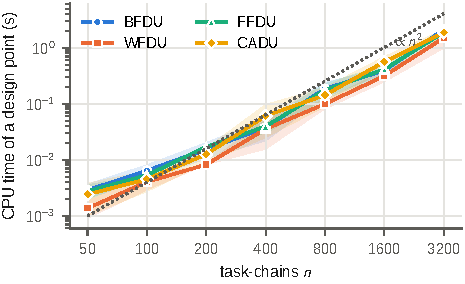
\includegraphics[width=\columnwidth]{figures/scaling}
\caption{CPU time of a design point against the number of task-chains
(log-log; dotted: slope 2).}
\label{fig:scaling}
\end{figure}

\begin{keybox}{Main findings}
\begin{itemize}[leftmargin=1em]
\item No simulated delay exceeded its bound: 3377 network flows (all four
TSN mechanisms) and 9000 task-chains simulated as a whole system, where
the end-to-end bounds are reached exactly or within 1\,\% (RQ0).
\item With consolidation, the packing rules are 2.3 to 2.9\,\% above the
optimal allocation on average, and proven optimal in 81\,\% of the
instances of up to 300 task-chains, in milliseconds; simulated annealing needs seconds to come as
close on the default platform, and a genetic algorithm does not; on the
domain platform and with slow zones, a genetic algorithm run for tens of
seconds recovers most of the gap of the packing rules, and the exact
formulation all of it (RQ1).
\item Communication awareness removes about two thirds of the inter-ECU
communications for a third more cores (RQ2).
\item ATS removes the burst growth of rings; frame replication for the
replicated task-chains costs little bandwidth and deadline satisfaction;
strict LET cuts the network bounds by 15 to 19\,\% but costs 30 points of
deadlines with \FFDU\ and 16 with \CADU\ (RQ3).
\item Memory contention can add half the cores of a packed mapping, much
less for a communication-aware one (RQ4).
\item Each core bought at the SOP buys about half a software update; the
margin after the first update is set by the design cap, not by the
provisioning (RQ6).
\item The method maps domain, hybrid and distributed platforms as well,
within 4.7\,\% of the optimum on the domain platform and 1.2\,\% on the
hybrid one (RQ1); both need about a core less than the zonal platform,
and a distributed one holds only half the applications of 300
task-chains (RQ7).
\item Consolidation saves 0.9 to 1.9 cores and the local search adds 4 to
13 points of task-chains on time; putting all free software on the
central computer costs cores, communications and 7 points on time;
whole task-chains fail under memory contention (RQ8).
\item These conclusions hold when each assumption of the generator is
set to a lower or a higher value (RQ9).
\end{itemize}
\end{keybox}
